% SPDX-License-Identifier: CC-BY-SA-4.0
% Author: Matthieu Perrin
% Part: 
% Section: 
% Sub-section: 
% Frame: 

\begingroup

\begin{frame}{Actions d'un AFN}

  \tfBlock[top=-3mm]{Définition -- Action (ou \structure{calcul}, ou \structure{déplacement})}{
    Soit $A=\langle \Sigma, Q, I, F, \rightarrow \rangle$ un AFN. \\
    Les \structure{actions}  de $A$ composent une relation binaire \alert{$\leadsto_A$} sur les configurations.\\
    On a \alert{$\langle u, q\rangle \leadsto_A \langle v, q'\rangle$} ssi il existe \alert{$a \in \Sigma\cup\{\varepsilon\}$} tel que
    \begin{enumerate}
    \item \alert{$u=a v$} et
    \item \alert{$q \xrightarrow{a} q'$}.
    \end{enumerate}
    On note \alert{$\leadsto_A^\star$} \structure{la fermeture transitive et réflexive de $\leadsto_A$}.
    
    \vspace{1mm}On notera \alert{$C \leadsto C'$} et \alert{$C \leadsto^\star C'$} si $A$ est clair d'après le contexte.
  }

  \tfExampleBlock[bottom]{Exemple : $\langle bbc, 3\rangle \leadsto^\star \langle \varepsilon, 2\rangle$}{
    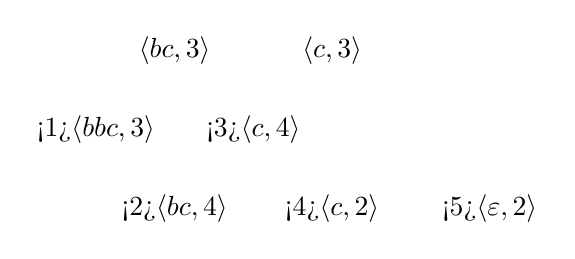
\begin{tikzpicture}
      \tikzset{leadsto/.style={decorate, decoration={snake, amplitude=.5mm, segment length=2mm, post=lineto, post length=1mm},->,},}
      \node (c1) at (0.0,1.0) {\example<1>{$\langle bbc,         3\rangle$}};
      \node (c2) at (1.0,2.0) {            $\langle bc,          3\rangle$};
      \node (c3) at (1.0,0.0) {\example<2>{$\langle bc,          4\rangle$}};
      \node (c4) at (3.0,2.0) {            $\langle c,           3\rangle$};
      \node (c5) at (2.0,1.0) {\example<3>{$\langle c,           4\rangle$}};
      \node (c6) at (3.0,0.0) {\example<4>{$\langle c,           2\rangle$}};
      \node (c7) at (5.0,0.0) {\example<5>{$\langle \varepsilon, 2\rangle$}};

      \smPath[                     ] (c1) edge[leadsto] (c2);
      \smPath[\smExample<1|handout>] (c1) edge[leadsto] (c3);
      \smPath[                     ] (c2) edge[leadsto] (c4);
      \smPath[                     ] (c2) edge[leadsto] (c5);
      \smPath[\smExample<2|handout>] (c3) edge[leadsto] (c5);
      \smPath[\smExample<3|handout>] (c5) edge[leadsto] (c6);
      \smPath[\smExample<4|handout>] (c6) edge[leadsto] (c7);
    \end{tikzpicture}
  }

  \tf[y=-22.5mm, x=10mm]{
    \begin{smArray}[size=7mm]
      \smCell[\smNone]{}
      \smCell[\smExample<1> ]{b} \smHead<1|handout>  [example]
      \smCell[\smExample<-2>]{b} \smHead<2>          [example]
      \smCell[\smExample<-4>]{c} \smHead<3,4>        [example]
      \smCell[\smNone]{}         \smHead<5>          [example]
    \end{smArray}
  }

  \tf[bottom, x=.4\textwidth]{
    \begin{tikzpicture}[smAutomaton]\small
      \smState[\smInitial                          ] (1) at (0.0,1.5) {$1$}; 
      \smState[\smAccepting\smExample<4->          ] (2) at (1.5,1.5) {$2$}; 
      \smState[\smInitialAbove\smExample<1|handout>] (3) at (0.0,0.0) {$3$}; 
      \smState[\smExample<2,3>                     ] (4) at (1.5,0.0) {$4$}; 

      \smPath                        (1) edge             node       {$a$}           (2);
      \smPath                        (1) edge[loop above] node       {$a$}           (1);
      \smPath[\smExample<1|handout>] (3) edge             node[swap] {$b$}           (4);
      \smPath                        (3) edge[loop left ] node       {$b$}           (3);
      \smPath[\smExample<2>        ] (4) edge[loop right] node       {$b$}           (4);
      \smPath[\smExample<4>        ] (2) edge[loop above] node       {$c$}           (2);
      \smPath[\smExample<3>        ] (4) edge             node[swap] {$\varepsilon$} (2);
    \end{tikzpicture}
  }

\end{frame}

\endgroup
